\documentclass[../finalreport.tex]{subfiles}

\begin{document}

\subsubsection{Formule explicite, faisabilité numérique}

\par Comme en section \ref{section_1_4}, plaçons-nous dans le cas particulier où la variable connue par l'initié est $L = \ln \left( S_T^{1} \right) - \ln \left( S_T^{2} \right)$ (toutes les hypothèses techniques nécessaires à l'établissement de la solution du problème d'optimisation sont alors vérifiées), et où les paramètres $b, \sigma$, et $r$ du modèle sont constants.

\par Alors (cf. \cite{art5}), 

\begin{displaymath}
Z \left( t \right) = \dfrac{\prod\limits_{j = 1}^{n} \sum\limits_{k_j = 0}^{+ \infty} \dfrac{e^{- {\kappa}_j \left( T - t\right)}}{\sqrt{2 \pi {\Sigma}_t}} {\displaystyle \int_{{\left( F_{t, T, k_j}\right)}^n}} e^{\left( \frac{- \left( L - m_t - \sum\limits_{j = 1}^{n} \sum\limits_{l_j = 1}^{k_j} \ln \left( \frac{1 + {\sigma}_{i_1, j}}{1 + {\sigma}_{i_2, j}} \right) \left( t_{j, l_j} \right) \right)^2}{2 {\Sigma}_t} \right)} \prod d t_{j, l_j}}{\prod\limits_{j = 1}^{n} \sum\limits_{k_j = 0}^{+ \infty} \dfrac{e^{- {\kappa}_j T}}{\sqrt{2 \pi {\Sigma}_0}} {\displaystyle \int_{{\left( F_{0, T, k_j}\right)}^n}} e^{\left( \frac{- \left( L - m_0 - \sum\limits_{j = 1}^{n} \sum\limits_{l_j = 1}^{k_j} \ln \left( \frac{1 + {\sigma}_{i_1, j}}{1 + {\sigma}_{i_2, j}} \right) \left( t_{j, l_j} \right) \right)^2}{2 {\Sigma}_t} \right)} \prod d t_{j, l_j}}
\end{displaymath}

où

\begin{displaymath}
\begin{cases}
{\Sigma}_t &= \displaystyle \int_{s = t}^{T} \left\Vert \sigma_{1, 1} - \sigma_{2, 1} \right\Vert^2 ds \\
L - m_t &= \displaystyle \int_{s = t}^{T} \left( \underbrace{\sigma_{1, W}}_{\substack{\text{partie "brownienne"} \\ \text{(m premières composantes)} \\ \text{de } \sigma_1}} - \sigma_{2, W} \right) dW(s) + \int_{s = t}^{T} \ln \left( \frac{1 + \sigma_{1, N}}{1 + \sigma_{2, N}} \right) dN(s) \\
{\left( F_{t, T, k_j}\right)}^n &= \left\lbrace \left( t_{j, l_j} \right)_{\substack{1\leq j\leq n \\ 1\leq l_j\leq k_j}} \in \mathbb{R}^{k_1 + ... + k_n}, t \leq t_{j, l_1} \leq ... \leq t_{j, l_{k_j}} \leq T \text{ pour } 1 \leq j \leq n \right\rbrace
\end{cases}
\end{displaymath}

\par Ainsi, nous avons une expression "close" pour exprimer la richesse de l'initié et du non-initié : nous pouvons calculer $Y_0$ en explicitant la solution de l'exponentielle de Doléans-Dade selon la formule (\ref{doleans_explicite}), puis $Y$ via la formule $Y = \frac{Y_0}{Z}$ avec $Z$ exprimé ci-dessus. Cependant, la complexité de l'expression de $Z$ le rend difficile à exploiter. En particulier, il s'agit de sommer une infinité de termes intégrés sur des hypertétraèdres en dimension de plus en plus grande, ce qui complique l'implémentation informatique.

\par L'analyse heuristique qui suit a pour but de justifier qu'il est nécessaire de calculer un grand nombre de termes dans la somme pour avoir un résultat précis, notamment lorsque $t \to T$. Nous allons estimer le premier terme de la somme dans un cas particulier et constater que $Z \left( t \right) $ tend vers $0$ exponentiellement vite lorsque $t \to T$, alors que - comme dans la partie précédente - nous nous attendons à un phénomène d'explosion lorsque $t \to T$ : nous imputons ce "paradoxe" au fait qu'un seul terme ne suffit pas à estimer $Z$, d'autant plus lorsqu'on étudie $t$ proche de $T$.

\par Plaçons-nous dans le cadre encore plus simplifié d'un marché avec deux actifs risqués et un actif sans risque ($n = m =1$). Dans ce cas, le numérateur dans la formule précédente s'écrit :

\begin{displaymath}
Z_{\text{num}} \left( t \right) = \sum\limits_{k_j = 0}^{+ \infty} \dfrac{e^{- {\kappa} \left( T - t\right)}}{\sqrt{2 \pi {\Sigma}_t}} {\displaystyle \int_{{\left( F_{t, T, k_j}\right)}^1}} e^{\left( \frac{- \left( L - m_t - \sum\limits_{l_j = 1}^{k_j} \ln \left( \frac{1 + {\sigma}_{1, 2}}{1 + {\sigma}_{2, 2}} \right) \left( t_{1, l_j} \right) \right)^2}{2 {\Sigma}_t} \right)} \prod d t_{1, l_j}
\end{displaymath}

\par Regardons le premier terme de cette somme ($k_j = 1$):

\begin{displaymath}
Z_{\text{num}, 1} \left( t \right) =  \dfrac{e^{- {\kappa} \left( T - t\right)}}{\sqrt{2 \pi {\Sigma}_t}} {\displaystyle \int_{{\left( F_{t, T, 1}\right)}^1}} e^{\left( \frac{- \left( L - m_t - \ln \left( \frac{1 + {\sigma}_{1, 2}}{1 + {\sigma}_{2, 2}} \right) \left( t_{1, 1} \right) \right)^2}{2 {\Sigma}_t} \right)} \prod d t_{1,1}
\end{displaymath}

\par Or par définition, ${\left( F_{t, T, 1}\right)}^1 = \left[ t, T \right]$, i.e.

\begin{displaymath}
Z_{\text{num}, 1} \left( t \right) =  \dfrac{e^{- {\kappa} \left( T - t\right)}}{\sqrt{2 \pi {\Sigma}_t}} {\displaystyle \int_{s = t}^{T}} e^{\left( \frac{- \left( L - m_t - \ln \left( \frac{1 + {\sigma}_{1, 2}}{1 + {\sigma}_{2, 2}} \right) s  \right)^2}{2 {\Sigma}_t} \right)} ds
\end{displaymath}

\par Par définition, nous avons : 

\begin{displaymath}
	\begin{split}
	{\Sigma}_t &= \int_{s = t}^{T} \left\Vert \sigma_{1, 1} - \sigma_{2, 1} \right\Vert^2 ds \\
			   &= (T - t) \left\Vert \sigma_{1, 1} - \sigma_{2, 1} \right\Vert^2
	\end{split}
\end{displaymath}

\par et (cf. page 13):

\begin{displaymath}
	\begin{split}
	L - m_t &= \int_{s = t}^{T} \left( \sigma_{1, 1} - \sigma_{2, 1} \right) dW(s) + \int_{s = t}^{T} \ln \left( \frac{1 + \sigma_{1, 2}}{1 + \sigma_{2, 2}} \right) dN(s) \\
	&= \left( \sigma_{1, 1} - \sigma_{2, 1} \right) \left( W\left(T\right) -  W\left(t\right) \right) + \ln \left( \frac{1 + \sigma_{1, 2}}{1 + \sigma_{2, 2}} \right) \sum\limits_{t < s \leq T} \Delta N(s)
	\end{split}
\end{displaymath}

\par Nous pouvons supposer qu'il n'y a pas de saut en $T$ dans le processus $N$, donc que pour $t$ suffisamment proche de $T$ (l'analyse qui suit suppose $t$ après le dernier saut),

\begin{displaymath}
\sum\limits_{t < s \leq T} \Delta N(s) = 0
\end{displaymath}

\par i.e.

\begin{displaymath}
L - m_t  = \left( \sigma_{1, 1} - \sigma_{2, 1} \right) \left( W\left(T\right) -  W\left(t\right) \right)
\end{displaymath}

\par ce qui nous permet de simplifier 

\begin{displaymath}
Z_{\text{num}, 1} \left( t \right) =  \dfrac{e^{- {\kappa} \left( T - t\right)}}{\sqrt{2 \pi {(T - t) \left\Vert \sigma_{1, 1} - \sigma_{2, 1} \right\Vert^2}}} {\displaystyle \int_{s = t}^{T}} e^{\left( \frac{- \left( \left( \sigma_{1, 1} - \sigma_{2, 1} \right) \left( W\left(T\right) -  W\left(t\right) \right) - \ln \left( \frac{1 + {\sigma}_{1, 2}}{1 + {\sigma}_{2, 2}} \right) s  \right)^2}{2 {(T - t) \left\Vert \sigma_{1, 1} - \sigma_{2, 1} \right\Vert^2}} \right)} ds
\end{displaymath}

\par Notons $\alpha = \sigma_{1, 1} - \sigma_{2, 1}$ et $\beta = \ln \left( \frac{1 + {\sigma}_{1, 2}}{1 + {\sigma}_{2, 2}} \right)$, alors à une constante multiplicative près (ne dépendant pas de $t$),

\begin{displaymath}
Z_{\text{num}, 1} \left( t \right) =  \dfrac{e^{- {\kappa} \left( T - t\right)}}{\sqrt{(T - t)}} {\displaystyle \int_{s = t}^{T}} e^{\left( \frac{- \left( \alpha \left( W\left(T\right) -  W\left(t\right) \right) - \beta s  \right)^2}{2 {(T - t) \alpha^2}} \right)} ds
\end{displaymath}

\par Expérimentalement, nous constatons que ce terme converge vers 0 lorsque $t$ tend vers $T$. 
\par Heuristiquement, cela peut se "justifier" par l'approximation $s = T$ dans l'intégrale lorsque $t$ et proche de $T$ : 

\begin{displaymath}
	\begin{split}
	Z_{\text{num}, 1} \left( t \right) &\sim  \dfrac{e^{- {\kappa} \left( T - t\right)}}{\sqrt{(T - t)}} (T - t) e^{\left( \frac{- \left( \alpha \left( W\left(T\right) -  W\left(t\right) \right) - \beta T  \right)^2}{2 {(T - t) \alpha^2}} \right)} \\
	&= \sqrt{(T - t)} e^{- {\kappa} \left( T - t\right)}  e^{ - \frac{\alpha^2 \left( W\left(T\right) -  W\left(t\right) \right)^2}{2 (T - t) \alpha^2}} e^{ \frac{2 \left( W\left(T\right) -  W\left(t\right) \right) \beta T}{2 (T - t) \alpha^2}} e^{ - \frac{\beta^2 T^2}{2 (T - t) \alpha^2}}
	\end{split}
\end{displaymath}

\par Nous remplaçons enfin les mouvements browniens par leur espérance : $W\left(T\right) -  W\left(t\right) \sim 0$ et $  \left( W\left(T\right) -  W\left(t\right) \right)^2 \sim (T - t)$ : 
\begin{displaymath}
	\begin{split}
	Z_{\text{num}, 1} \left( t \right) &\sim \sqrt{(T - t)} e^{- {\kappa} \left( T - t\right)}  e^{ - \frac{1}{2}} e^{0} e^{ - \frac{\beta^2 T^2}{2 (T - t) \alpha^2}} \\
	& \xrightarrow[t \to T]{} 0 \quad \text{exponentiellement vite}
	\end{split}
\end{displaymath}

\par Voici quelques représentations de l'évolution de $Z_{\text{num}, 1}$ (implémentées numériquement en \emph{Python}) pour différentes valeurs de $\alpha$ et $\beta$.
 
\begin{figure}[H]
  \centering
    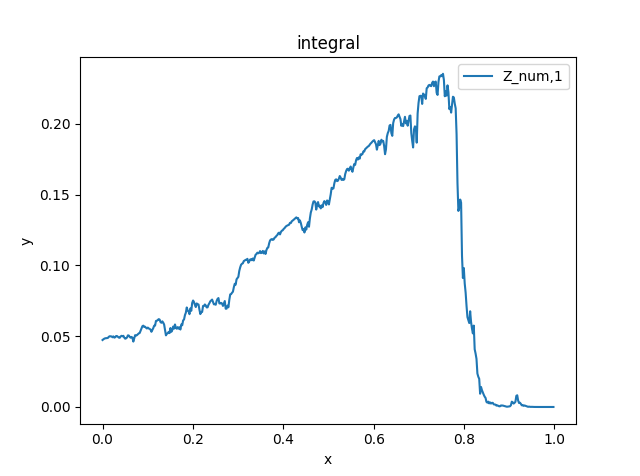
\includegraphics[width=0.7\textwidth]{images/paradox_1.png}
  \caption{$Z_{\text{num}, 1}$}
\end{figure}

\begin{figure}[H]
  \centering
    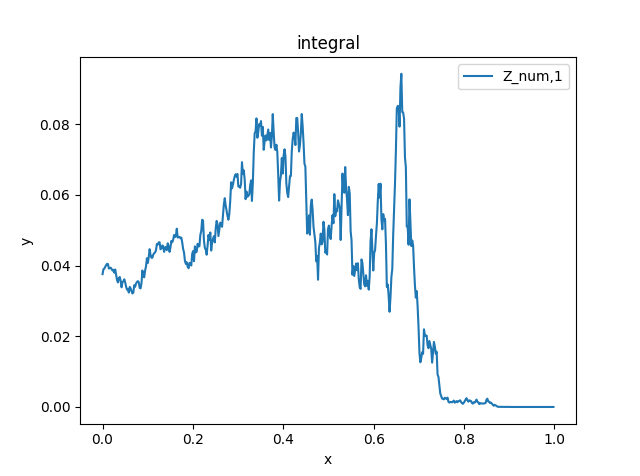
\includegraphics[width=0.7\textwidth]{images/paradox_2.png}
  \caption{$Z_{\text{num}, 1}$}
\end{figure}

\par Nous y constatons que le processus "s'affaisse" bien avant $T$ (vers $t \simeq 0.7$) ce qui traduit que plus de termes sont nécessaires pour estimer précisément $Z$ autour de $T$, et surtout après le dernier saut.

\subsubsection{Simulations numériques}

\par Comme dans la section \ref{section_1_4}, nous avons implémenté ces formules en \emph{Python}. Afin d'avoir des simulations précises, le phénomène souligné précédemment nous conduirait naturellement à choisir un modèle dans lequel il y a un certain nombre de sauts, afin de réduire cette "fenêtre d'affaissement" après le dernier saut. Cependant, la formule définissant $Z$ fait aussi intervenir un terme en $e^{\kappa t}$ donc il faut veiller à ce que l'intensité du processus de Poisson ne soit pas trop grande afin de ne pas créer un $Z$ qui explose avant de chuter vers $0$. Ainsi, il faut choisir avec attention les paramètres du modèle afin que les calculs soient relativement précis tout en étant exploitables.

\par Dans notre simulation (\emph{simulations\_jump\_model.py}), 
\begin{displaymath}
\begin{cases}
T &= 1 \\
A &= 0.9 \\
m &= n = 1 \quad \text{donc } d = 2 \\
r &= 0.25 \\
\kappa &= 5 \\
b &= \begin{bmatrix}
		0.25 & 0.01
	\end{bmatrix} \\
\sigma &= \begin{bmatrix}
			-0.05 & 0.01 \\
			0.07 & 0.01
		  \end{bmatrix}
\end{cases}
\end{displaymath}

\par Et nous calculons dans $Z$ les deux premiers termes de la somme. Les prix évoluent de la manière suivante :
\begin{figure}[H]
  \centering
    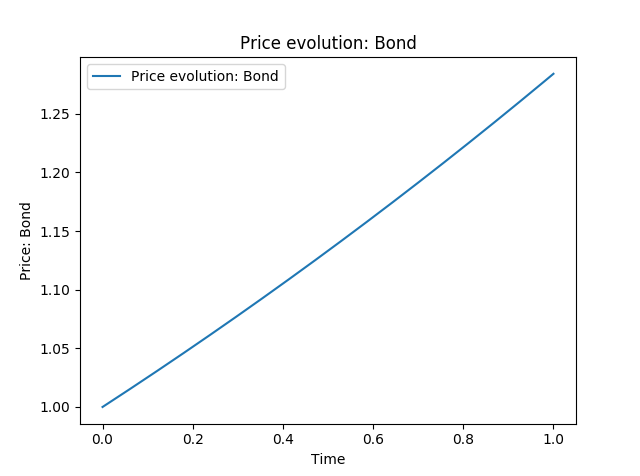
\includegraphics[width=0.7\textwidth]{images/simulation_2/price_0.png}
  \caption{prix de l'actif sans risque}
\end{figure}

\begin{figure}[H]
  \centering
    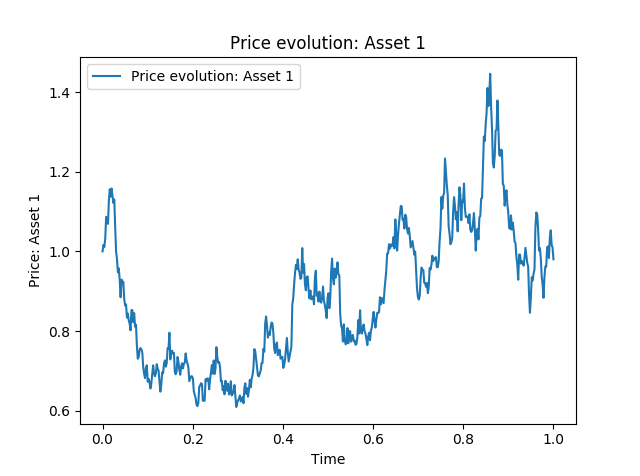
\includegraphics[width=0.7\textwidth]{images/simulation_2/price_1.png}
  \caption{prix de l'actif risqué 1}
\end{figure}

\begin{figure}[H]
  \centering
    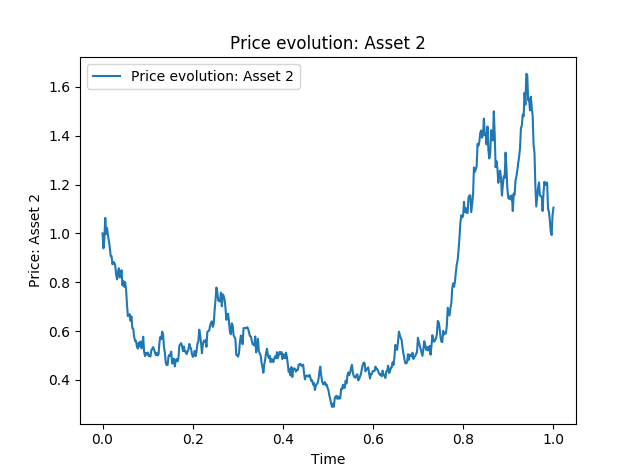
\includegraphics[width=0.7\textwidth]{images/simulation_2/price_2.png}
  \caption{prix de l'actif risqué 2}
\end{figure}

\par La valeur de la variable connue par l'initié est $L = 0.22$. Le processus $Z$ vaut ensuite :

\begin{figure}[H]
  \centering
    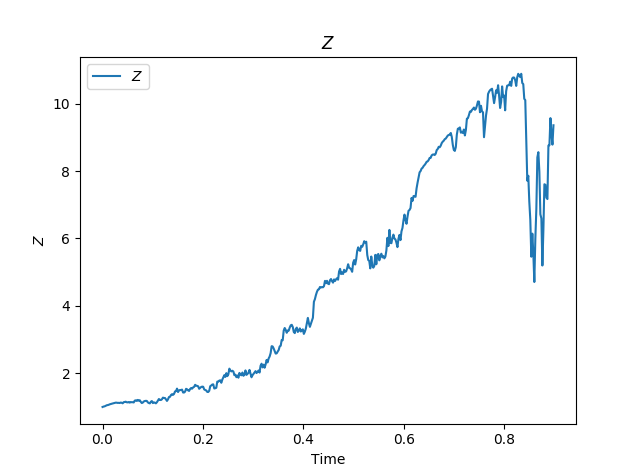
\includegraphics[width=0.7\textwidth]{images/simulation_2/Z.png}
  \caption{$Z$ sur $\left[0; A \right]$}
\end{figure}

\par Nous constatons que, comme voulu, le choix des paramètres permet à l'approximation numérique du processus $Z$ de diverger lorsque $t$ se rapproche de $T$. Nous pouvons enfin représenter l'évolution comparé de la richesse des deux agents :

\begin{figure}[H]
  \centering
    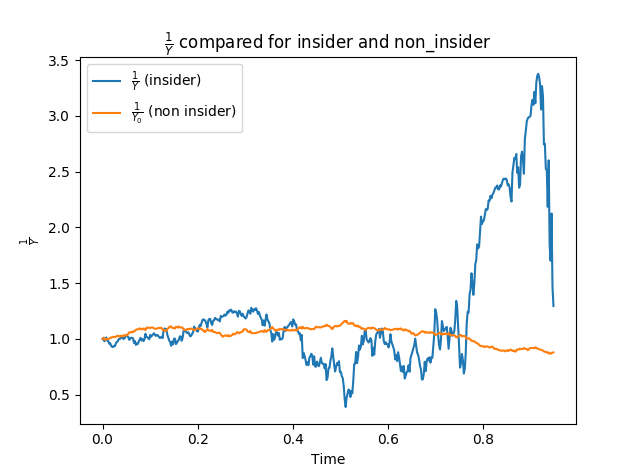
\includegraphics[width=0.7\textwidth]{images/simulation_2/compared_wealths.png}
  \caption{$\frac{1}{Y_0}$ et $\frac{1}{Y}$ sur $\left[0; A \right]$}
\end{figure}

\par Ainsi, dans cette situation encore, l'information supplémentaire conférée à l'initié lui permet d'établir une meilleure stratégie que le non-initié.

\end{document}